\section{Cyclic Processes with an Ideal Gas}

\begin{comment}
This lab is more of a worksheet than it is a lab.  But I've used versions of if in my 132 classes for a while, so I thought it was time to include it here in the lab manual for others as well.  --Matt Trawick, 6/2015

Activity 1 is straightforward practice with the ideal gas law, Q, E, and W.
Activity 2 works through isothermal and adiabatic expansions.
Activity 3 is the only part that actually works to introduce a new topic, as opposed to practicing something the students are presumed to have seen before.

In the past, I've done Activities 1 and 2 on different days, as two different worksheets.

\end{comment}

\makelabheader %(Space for student name, etc., defined in master.tex)

\vspace{0.1in}
\textbf{Objective} 

In this lab, you will examine an ideal gas going through a cycle in which it is compressed and expanded, eventually returning to its initial state.  During this time, thermal energy enters and leaves the gas, and useful work can be extracted from it.  These cycles are the basis of refrigerators (which put work into a system to move heat energy from something cold to something hot) and heat engines (which move heat energy from something hot to something cold, extracting useful work along the way.

\textbf{Activity 1: A Rectangular Cycle}

\begin{wrapfigure}[3]{r}{0.4\textwidth}
    \vspace{-0.2 in}
    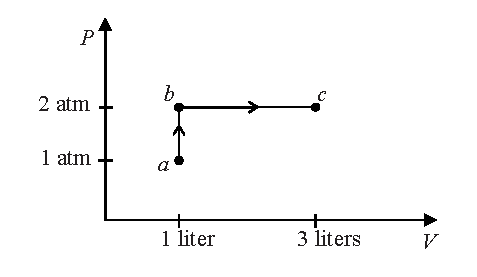
\includegraphics[width=0.4\textwidth]{ideal_gas_cycles/square_cycle1.eps}
\end{wrapfigure}

We start with a sample of 1 liter of nitrogen ($\textrm{N}_2$) gas, at temperature $T_a = 300$ K and pressure $P_a = 10^5$ N/m$^2$ (about 1 atm).

(a) Find the number of moles $n$ of the gas.
\vspace{1.0in}

(b) As the figure shows, the gas is heated at constant volume from point $a$ to point $b$, then heated at constant pressure to point $c$.  Find the temperatures $T_b$ and $T_c$.  
\vspace{1.4in}

(c) Find the change in the internal energy $E$ for the gas for the processes $a \rightarrow b$ and $b \rightarrow c$.  (Call these $\Delta E_{ab}$ and $\Delta E_{bc}$.)
\vspace{1.5in}

\pagebreak
(d) Find the work done on the gas for each process, $W_{ab}$ and $W_{bc}$.  
\vspace{1.3in}

(e) Find theheat added to the gas for each process, $Q_{ab}$ and $Q_{bc}$.  
\vspace{1.3in}

\begin{wrapfigure}[3]{r}{0.4\textwidth}
  \vspace{-0.4 in}
  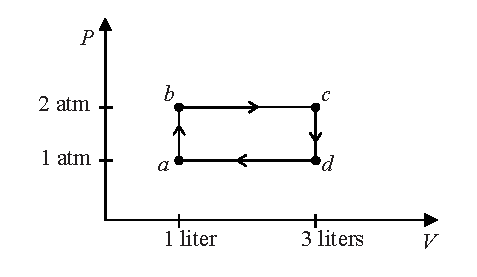
\includegraphics[width=0.4\textwidth]{ideal_gas_cycles/square_cycle2.eps}
\end{wrapfigure}

Now the gas is cooled at a constant volume from point $c$ to point $d$, and cooled at constant pressure from point $d$ back to point $a$.  

(f) Find the temperature $T_d$ at point $d$.
\vspace{0.9in}

(g) Complete the following table:

%For fixed width columns:
%These are now defined in master.text:
%\newcolumntype{L}[1]{>{\raggedright\arraybackslash}p{#1}}
%\newcolumntype{C}[1]{>{\centering\arraybackslash}p{#1}}
%\newcolumntype{R}[1]{>{\raggedleft\arraybackslash}p{#1}}

\vspace{0.1 in}
\renewcommand{\arraystretch}{2.0}
\begin{tabular}{| C{1in} |C{1in} | C{1in} | C{1in} |}
\hline
& $\Delta E$ & $W$ & $Q$ \\ \hline
$a \rightarrow b$ & & & \\ \hline
$b \rightarrow c$ & & & \\ \hline
$c \rightarrow d$ & & & \\ \hline
$d \rightarrow a$ & & & \\ \hline
\hline
NET: & & & \\ \hline
\end{tabular}
\renewcommand{\arraystretch}{1.0}

\vspace{0.3in}

\pagebreak
\textbf{Activity 2: A Carnot Cycle}

As in the previous activity, we start with 1 liter of ($\textrm{N}_2$) gas at temperature $T_a = 300$ K and pressure $P_a = 10^5$ N/m$^2$.   As you found before, this gives $nR=\frac{1}{3}$ J/K, or $n=0.0401$ moles.  We'll heat the gas to a maximum temperature of 1800 K again, but here we do so in one step, a single adiabatic compression, as shown in process $a \rightarrow b$ of the figure below.

\begin{minipage}{0.45\textwidth}
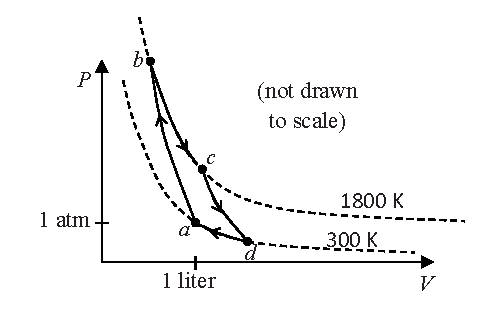
\includegraphics[width=1.0\textwidth]{ideal_gas_cycles/carnot_cycle.eps}
\end{minipage}
\begin{minipage}{0.55\textwidth}
\vspace{0.1 in}
\renewcommand{\arraystretch}{2.0}
\begin{tabular}{| C{0.6in} | C{0.6in} | C{0.6in} | C{0.6in} | C{0.6in} |}
\hline
& $P$ & $V$ & $NR$ & $T$ \\ \hline
$a$ & $10^5$ Pa & $10^{-3}$ m$^3$ & $\frac{1}{3}$ J/K & 300 K \\ \hline
$b$ &                  &                            & $\frac{1}{3}$ J/K & 1800 K \\ \hline
$c$ &                  &                            & $\frac{1}{3}$ J/K & 1800 K \\ \hline
$d$ &                  &                            & $\frac{1}{3}$ J/K & 300 K \\ \hline
\end{tabular}
\renewcommand{\arraystretch}{1.0}
\end{minipage}

(a) Recalling that $PV^\gamma$ is constant for an adiabatic process, where $\gamma = C_P / C_V$, what is the final volume $V_b$?  (Answer: $V_b=1.134 \times 10^{-5}$ m$^3$.)  
\vspace{1.8in}

(b) What are $\Delta E_{ab}$, $W_{ab}$, and $Q_{ab}$?  Go ahead and start filling out the table on the next page if you like.  Also, the table just above may help you keep your thoughts organized.
\vspace{1.8in}

\pagebreak
(c) In the process $b \rightarrow c$, the gas is expanded isothermally to a new volume, $V_c=1.6918 \times 10^{-5}$ m$^3$.  Calculate $\Delta E_{bc}$, $W_{bc}$, and $Q_{bc}$ for this process.  (This particular value for $V_c$ makes the numbers in the table turn out pretty.  You’ll see.)
\vspace{1.6in}

(d) Now the gas is expanded adiabatically back to $T_d=300$ K.  Find $V_d$, and also find  $\Delta E_{cd}$, $W_{cd}$, and $Q_{cd}$.
\vspace{2.0in}


(e) Finally, the gas is compressed isothermally back to $V_a$.  Find $\Delta E_{da}$, $W_{da}$, and $Q_{da}$.  
\vspace{1.6in}



(f) If you haven’t done so already, complete the following table:
\vspace{0.1 in}

\renewcommand{\arraystretch}{2.0}
\begin{tabular}{| C{1in} |C{1in} | C{1in} | C{1in} |}
\hline
& $\Delta E$ & $W$ & $Q$ \\ \hline
$a \rightarrow b$ & & & \\ \hline
$b \rightarrow c$ & & & \\ \hline
$c \rightarrow d$ & & & \\ \hline
$d \rightarrow a$ & & & \\ \hline
\hline
NET: & & & \\ \hline
\end{tabular}
\renewcommand{\arraystretch}{1.0}

\pagebreak
\textbf{Activity 3: Comparing the Two Cycles}

Compare the table at the end of Activity 1 for a rectangular cycle with the table you just completed in Activity 2 for a ``Carnot cycle.'' 

(a)  What is the net work $W$ done by the gas in each case?

\begin{displaymath}
\hspace{-0.5in} W_{\substack{\textrm{NET} \\ \\ \textrm{RECT}}} =
\hspace{2in} W_{\substack{\textrm{NET} \\ \\ \textrm{CARNOT}}} =
\end{displaymath}


(b)  What is the total heat $Q_{IN}$ put into the gas from the hot reservoir?

\begin{displaymath}
\hspace{-0.5in} \left| Q_{\substack{\textrm{IN} \\ \\ \textrm{RECT}}} \right| =
\hspace{2in} \left| Q_{\substack{\textrm{IN} \\ \\ \textrm{CARNOT}}} \right|=
\end{displaymath}


(c) What is the total heat $Q_{OUT}$ dumped out of the gas into the cold reservoir in each process?

\begin{displaymath}
\hspace{-0.5in} \left| Q_{\substack{\textrm{OUT} \\ \\ \textrm{RECT}}} \right| =
\hspace{2in} \left| Q_{\substack{\textrm{OUT} \\ \\ \textrm{CARNOT}}} \right|=
\end{displaymath}

(d)  Which heat engine is more efficient?  That is, which heat engine does the most work per ton of coal burned?





